%%%%%%%%%%%%%%%%%%%%%%%%%%%%%%%%%%%%%%%%%%%%%%%%%%%%%%%%%%%%% 
\begin{abstract}
In this paper we introduce and investigate an adaptive direct volume rendering (DVR) method for real-time visualization of cardiac 3D ultrasound.  DVR is commonly used in cardiac ultrasound to visualize interfaces between tissue and blood. However, this is particularly challenging with ultrasound images due to variability of the signal within tissue as well as variability of noise signal within the blood pool. Standard DVR involves a global mapping of sample values to opacity by an opacity transfer function (OTF). While a global OTF may represent the interface correctly in one part of the image, it may result in tissue dropouts, or even artificial interfaces within the blood pool in other parts of the image. In order to increase correctness of the rendered image, the presented method utilizes blood pool statistics to do regional adjustments of the OTF. The regional adaptive OTF was compared with a global OTF in a dataset of apical recordings from 18 subjects. For each recording, three renderings from standard views (apical 4-chamber (A4C), inverted A4C (IA4C) and mitral valve (MV)) were generated for both methods, and each rendering was tuned to the best visual appearance by a physician echocardiographer. For each rendering we measured the mean absolute error (MAE) between the rendering depth buffer and a validated left ventricular segmentation. The difference $d$ in MAE between the global and regional method was calculated and t-test results are reported with significant improvements for the regional adaptive method ($\bar{d}_{A4C} = 1.5 \pm 0.3$ mm, $\bar{d}_{IA4C} = 2.5 \pm 0.4$ mm, $\bar{d}_{MV} = 1.7 \pm 0.2$  mm, d.f. $= 17$, all $p<0.001$). This improvement by the regional adaptive method was confirmed through qualitative visual assessment by an experienced physician echocardiographer who concluded that the regional adaptive method produced rendered images with fewer tissue dropouts and less spurious structures inside the blood pool in the vast majority of the renderings. The algorithm has been implemented on a GPU,  running an average of 16 fps with a resolution of 512x512x100 samples (Nvidia GTX460).
\end{abstract}

\graphicspath{{./Paper4/img/}}

\section{Introduction}
Direct volume rendering (DVR)\cite{Levoy1988} is commonly used in cardiac ultrasound to visualize interfaces between tissue and blood\cite{steen1994, Rabben2010, kiss2010}. DVR has the advantage over other methods like 2D-slicing that it presents a large part of the volumetric data in a single view. Figure \ref{fig:dvr}a presents such a volume rendering of a high quality cardiac ultrasound volume. Anatomical structures of special interest are highlighted; the left ventricle (LV), the mitral valve which separates LV from the left atrium (LA), and the interventricular septum which separates the LV from the right ventricle (RV). As can be seen, interpreting cardiac ultrasound data is difficult and requires a lot of training. Clear tissue-blood boundaries are therefore of great importance. However, this is challenging to achieve with ultrasound images due to variability of the signal within tissue as well as variability of noise signal within the blood pool.
\begin{figure}  
\begin{center}
\begin{minipage}[b]{0.5\linewidth}\centering
\includegraphics[height=1\textwidth]{vr_cardiac_high_quality.eps}\\
(a)
\end{minipage}%
\hspace{-5em}
\begin{minipage}[b]{0.6\linewidth}\centering
\includegraphics[height=0.4\textwidth]{otf2.eps}\\
(b)
\end{minipage} 
\end{center}
\caption[example] { \label{fig:dvr}  a). An example of direct volume rendering (DVR) of cardiac ultrasound. Highlighted anatomical structures are: The left ventricle (LV), the right atrium (RA), mitral valve and the interventricular septum.  b). Shows two opacity transfer functions (OTF) with a fuzzy transition between voxels excluded from (values below $\tau$) or included in the rendering (values above $\tau$). Adjusting $\tau$ (blue arrow) will either include or exclude more data.}
\end{figure} 
%DVR is based on a physical model of light moving through a gaseous medium, and for simplicity, only absorption and emission along each ray are considered in its standard formulation. 

At the core of DVR, optical properties (colour and opacity) are derived from a transfer function and integrated along rays of light. One ray for each pixel in the final image. Applying the transfer function is also known as classification since features are visually separated through assignment of different colours and opacities. On the other hand, selecting a transfer function with low classification error is considered a challenge and will always be related to the data at hand \cite{pfister2002transfer}. Figure \ref{fig:dvr}b shows an example of a monotonically increasing opacity transfer function (OTF) for cardiac ultrasound DVR. Unlike other medical imaging modalities like CT and MR, cardiac ultrasound data are assumed to consist of only two classes; tissue and the blood pool signal. Tissue is expected to have higher intensity than blood, but in practice the two class-distributions overlap. The OTF in Figure \ref{fig:dvr}b is therefore designed to give a fuzzy threshold between samples excluded from and samples included in the rendering. Selecting the right threshold, as for transfer functions design in general, is therefore a challenge in cardiac ultrasound visualization.   

There are several reasons for the overlap between tissue and blood pool signal in ultrasound images. Sidelobes of the ultrasound beam results in signal from off-beam structures (clutter noise). Speckle pattern, caused by interference between point scatterers results in high signal variance in homogeneous regions. Multiple reflections between tissue structures (reverberations) causes false echoes. Distortion of the ultrasound wave front caused by varying speed of sound in inhomogeneous tissue (aberrations) reduce the signal amplitude. Interfaces of high reflectivity (lungs, ribs and calcifications) and how tissue layers are aligned with the ultrasound beam result in drop-outs and varying tissue signal. Attenuation of the ultrasound signal with depth gives high variation in tissue intensity across the volume. While an optimal global OTF may represent the tissue-blood interface correctly in one part of the image, the high variation in tissue intensities may result in tissue dropouts, or even artificial interfaces within the blood pool in other parts of the image. The latter artefact is visible in the upper part of LV in Figure \ref{fig:dvr}a. Figure \ref{fig:dvr}a also shows a large dropout in the lateral wall. These problems are to some extent solved by clipping, but standard clipping also has its limitations due to planar geometry. The curved shape of cardiac chambers calls either for other clipping geometries or a way to better assign high opacity to voxels associated with tissue and low opacity otherwise\cite{patent}.

A lot of work has been done in the visualization community to improve the results given by standard DVR. Special attention has been devoted to the problem of selecting the right transfer function\cite{Kindlmann1998, sereda2006visualization, wesarg2d, Woodring2009, Haidacher2010, correa2010visibility, Wang2011} and exploration of illustrative or non-photorealistic techniques to bring important information into focus\cite{viola2005, bruckner2006illustrative, Rezk-Salama2006, Malik2007, Bruckner2009}. Recently, Marchesin et al. \cite{marchesin2010} introduced a relevance function for feature enhancement in volume rendering. The paper differs from earlier contributions by also suggesting how to derive a relevance map without having any prior knowledge of voxel priorities. However, the use of local gradients as relevance indicators together with the per-ray constant opacity, yielding transparent renderings, makes it unsuitable for cardiac ultrasound. In our approach we adapt the ideas given by Marchesin et al. on how to do local opacity modulations, but with a relevance map better suited for cardiac ultrasound. For medical applications many adaptive and semi-adaptive DVR-like techniques have been proposed for enhancing anatomical structures\cite{borland2006volumetric, lindholm2010, 10.1109/TVCG.2006.100, Zhang2008}. For ultrasound, H\"{o}nigmann et al.\cite{Honigmann2003} proposed how to design a global adaptive OTF used to visualize volumetric fetal images. They also discussed the possibility of calculating one OFT for different regions in the rendering. Such a regional OTF can be derived from e.g. local edge detection or histograms. The method proposed in this paper regionally adapts the OTF by utilizing blood pool statistics derived from a real-time LV endocardial tracking algorithm\cite{orderud2006}. The purpose is to increase the correctness of the rendered image by reducing artificial tissue dropouts and spurious structures inside the blood pool.
%Our approach is highly influenced by this discussion, and in this paper we explore both regional and per-ray adaptation of the OTF.  

%For a visualization method to be applicable to cardiac ultrasound it needs be both fast and robust. Cardiac ultrasound is a real-time modality, so users expect immediate feedback on the display when moving the probe. In addition, the low SNR makes e.g. gradient calculation a challenge. Many of the proposed methods in the literature are based on semi-automatic transfer function design, depending on time-consuming user interaction. For automatic methods, boundaries are often expected to be related to the local gradient or histogram.


%limitations of the ultrasound imaging system causing a low signal-to-noise ratio (SNR)  
 
 

\section{Methods}
\subsection{Blood pool based regional adaptive opacity transfer function}
Selecting the correct global OTF for cardiac ultrasound visualization can be viewed as a global thresholding problem. Therefore we define the opacity threshold $\tau$ for a monotonically increasing OTF $\alpha$ as the highest sample value $v$ where all samples with lower value than $v$ will get zero opacity, $\tau = \max_{i}(v_i), \; \alpha(v_j)=0 \;\; \forall \; j<i$, hence they will be rendered transparent. 
As OTF we use a truncated polynomial:
\begin{equation}
\alpha(v) = \left\{
	\begin{array}{rl}
		0, &  v < \tau,\\
		\textrm{min}(a(v - \tau)^{\gamma}, k), & v \ge \tau.
	\end{array} \right.
\label{eq:otf}
\end{equation}
Global transparency is controlled by $a\in[0,\infty\rangle$, and in this paper $a=80$ has been selected to give a steep OTF. The truncation and gamma value are set to $k=0.5$ and $\gamma=2$ respectively. A second order polynomial has been selected instead of a standard linear OTF to increase the transparency of values near the opacity threshold. These values have a higher probability for being noise, and we let the opacity reflect this.

\begin{figure}  
\begin{center}
\begin{tabular}{cc}
\includegraphics[height=0.35\textwidth]{lot.eps} & 
\includegraphics[height=0.35\textwidth]{lotf_mesh2.eps}\\ % TODO Remove mesh and LOTF lable from this image
(a) & (b)
\end{tabular}
\end{center}
\caption[example] { \label{fig:lotf}  a) Shows ideal bimodal histograms of two density evolutions along ray $r_i$ and $r_j$. If we apply a global OTF (orange) on the given case we must select one ray were we want to separate tissue from blood. However, with a regional adapted OTF (green) we can find individual thresholds $\tau_r$ that minimizes the amount of misclassified samples along both rays. b) Estimated values of mean $\mu_r$ and standard deviation $\sigma_r$ inside the blood pool are used to regionally adjust the OTF. The regional opacity threshold $\tau_r = \mu_r + c\sigma_r$ is calculated for each ray $r$ intersecting a given left ventricular delineation.}
\end{figure} 
Since the global distributions of tissue and blood pool voxels usually overlap, adjusting $\tau$ will always involve a tradeoff between 
the number of true-positive and false-positive tissue voxels. If the opacity threshold is set too high, tissue surfaces will start to fall apart. However, if set too low, low level noise will get high opacity and the rendering will end before the actual tissue border is reached. Figure \ref{fig:lotf}a depicts the problem of having a global OTF (in orange). If rays $r_i$ and $r_j$ have noise ($n_r$) and tissue ($s_r$) levels given by $n_i$, $s_i$, $n_j$, $s_j$, with $n_i < s_i < n_j < s_j$, there are two obvious choices for $\tau$. The global opacity threshold $\tau$ can be selected as $n_i < \tau < s_i$ or $n_j < \tau < s_j$. The first choice makes $n_j$ occlude $s_j$, however the second choice will render $s_i$ transparent. This will result in an artificial hole in the final rendering along $r_i$. With our regional adaptive OTF, the idea is to let the opacity threshold $\tau$ vary across the framebuffer, making us able to define individual opacity thresholds for $r_i$ and $r_j$ (shown in green in Figure \ref{fig:lotf}a). 

In optical character recognition there has been a long tradition to utilize adaptive thresholding schemes to deal with variable background levels in 2D images\cite{Niblack1985}, thus maximizing the amount of foreground output. One simple adaptive method is based on estimates of regional statistics. The local image threshold $\tau_{x,y}$ is calculated as
\begin{equation}
\tau_{x,y} = \mu_{x,y} + c\sigma_{x,y},
\label{eq:niblack}
\end{equation}
where $c$ is a constant, and $\mu_{x,y}$ and $\sigma_{x,y}$ are mean and standard deviation estimates calculated in a window $w$ around (x,y). This yields what is known as a thresholding surface, where the method assumes that the foreground has higher expected value than the background inside $w$. Hence, foreground pixels are located above the thresholding surface.
	
To address our problem with high variability in tissue intensity in ultrasound images, we have designed a regional adaptive OTF by estimating the regional means and standard deviations of Equation \ref{eq:niblack} from the blood pool of the LV. The blood pool was delineated by a state-estimation algorithm capable of tracking the LV endocardium in real-time\cite{orderud2006}. The temporal state of the LV is returned by the framework as a time series of polygon meshes. How we utilize this information to do regional opacity adjustments is depicted in Figure \ref{fig:lotf}b. For a given frame we estimate the signal mean and standard deviation, $\mu_r$ and $\sigma_r$, along rendering ray $r$. Note that only the blood pool, the intersection between $r$ and the given LV delineation, is used to estimate $\mu_r$ and $\sigma_r$. The estimates are then used to calculate a regional opacity threshold $\tau_r$ given as
\begin{equation}
\tau_r=\mu_r+c\sigma_r, 
\label{eq:niblack_ray}
\end{equation}
where $c$ is a global constant adjusting $\tau_r$ around $\mu_r$ with a certain number of standard deviations. The local threshold $\tau_r$ together with Equation \ref{eq:otf} form our blood pool based regional adaptive OTF. Rays that do not intersect the given LV delineation are rendered using a global OTF.  


\subsection{Parameter space}
The proposed method in Equation \ref{eq:niblack_ray} introduces a parameter $c$, which controls how many standard deviations we want $\tau_r$ to deviate from the per-ray blood pool mean $\mu_r$. This parameter is clearly a substitution for the global opacity threshold, and adjusting $c$ will in the same way control the level of data visible in the rendered image. Setting $c = 0$ will render approximately $50\%$ of the blood pool samples transparent. Since we have a robust estimate of blood pool statistics, tissue signals are expected to have $\mu_{tissue} > \mu_r$ and $c > 0$ should be used.

The shape of the OTF is of great importance for the final appearance of a volume rendering. An OTF with a gentle slope will for instance result in a transparent look. In the proposed method we are more interested in the opacity threshold than the actual shape of the OTF, therefore we use the simple shifted and truncated second degree polynomial from Equation \ref{eq:otf} as a basis for the local OTF. Because it is a simple closed form expression, it can be used to quickly calculate on-the-fly opacity values.

For thresholding 2D images, the adaptive method in Equation \ref{eq:niblack} requires a window size that is directly related to the size of foreground objects. In our method, this window size depends on the ray-blood-pool intersection, and ideally no foreground (tissue) is included in the estimates. The regional opacity threshold $\tau_r$ is used along the full length of $r$, not just the intersection. Intersections with too few samples to give reliable statistics are rendered using a global OTF. 

\subsection{Spatial and temporal regularization}
Introducing adaptive visualization has some negative side effects. We trade spatial and temporal coherence in the presentation of anatomical structures for a better presentation of endocardial tissue. This does not pose any problems as long as the structure of interest along a given ray is associated with a value larger than the blood pool mean. Otherwise we risk rendering this structure transparent.
%The challenging part of estimating per-voxel relevance indicators in ultrasound data is to maintain spatial and temporal coherence of anatomical structures. 
%Since relevance in our method is proportional to intensity, structures of interest can be suppressed if they are not associated with a value larger than the blood pool estimate. 
The latter situation will often arise if e.g. the endocardium, mitral valve or papillary muscles are included in the estimated statistics. Given the properties of the real-time tracking framework, the two last structures, will to some extent, always be included. To exclude the endocardium we highly depend on a successful LV endocardial tracking. All segmentation algorithms will  be prone to errors and two regularization schemes have therefore been tested. First, we do spatial smoothing of estimates across neighbouring rays. This will constrain the regional adaptivity. Second, we do temporal smoothing over successive frames to reduce the per-frame adaptivity and potential flickering\cite{Peterscha2005}. The smoothing has been implemented as averaging filters on the framebuffer containing regional statistics. All regional adaptive renderings and statistics have been produced without any regularization in this paper. However the regularization schemes have been tested, and we will comment on how they perform.

%For each recording, a polygon model tracking the left ventricle has been provided by the AutoLVQ tool from GE Vingmed Ultrasound. With this information available, estimation of $\mu_r$ and $\sigma_r$ can be restricted to blood pool samples only. For rays intersecting the model, the opacity threshold $\tau_r$ is therefore a weighted sum between first and second order blood pool statistics along the ray. Other parts of the volume can be rendered using a global OTF.

\subsection{Rendering setup}
All renderings have been produced with Phong lighting and the data have been pre-smoothed with anisotropic diffusion\cite{perona1990scale, Steen}. %As common for 3D echocardiography, volume renderings are depth encoded for enhanced depth perception. 
For ray-casting it is normal to stop integrating when no significant transparency is left (known as early-ray-termination). We have chosen to terminate each ray when only $5 \%$ transparency is left. The rendering resolution has been set to 512x512x100.

\subsection{Measuring rendering accuracy}
As a measure of rendering accuracy, we have calculated the mean absolute error (MAE) between the rendering depth buffer (given by early-ray-termination) and a validated left ventrical segmentation. The reference segmentation was performed by an experienced physician echocardiographer using the AutoLVQ tool from GE Vingmed Ultrasound. The MAE measure will increase if the rendering contains tissue dropouts, or if spurious structures occlude endocardial tissue. A minimal MAE therefore exists when a majority of rays end their traversal near the tissue-blood border depicted by the reference segmentation. A view-aligned clipping plane has been applied to produce standard long-axis and mitral valve views, clipping away half of both the ventricle and the reference segmentation. Clipping of the volume from behind has also been applied to reduce the impact of non-terminated rays versus rays terminated by clutter noise.

\section{Results}\label{sec:res}

\subsection{Quantitative evaluation}
% table showing statistics
\begin{table}
\begin{center}
\begin{tabular}{c|ccc}
& Apical 4-chamber & Inverted apical 4-chamber & Mitral valve \\ \hline \\[-1.5ex]
$\bar{d}$ & $1.5 \pm 0.3$ mm & $2.5 \pm 0.4$ mm & $1.7 \pm 0.2$ mm\\ 
\end{tabular}
\end{center}
\caption[]{\label{tab:stat1} Statistics showing a significant improvement ($p < 0.001$, $\textrm{d.f.} = 17$) in mean absolute error (MAE) for the proposed regional adaptive method in three views. The variable $\bar{d}$ is the average difference plus-minus standard error between $\textrm{MAE}_{global}$ and $\textrm{MAE}_{regional}$ in 18 subjects.
%The null hypothesis that $\bar{d}$ is less than or equal to zero, i.e. $\textrm{MAE}_{global} \le \textrm{MAE}_{regional}$, has probability $p < 0.001$ for all views using t-statistics with $\textrm{d.f.} = 17$. 
All renderings are from end-diastole and were tuned to the best visual appearance by a physician echocardiographer.}
\end{table}
The global and regional adaptive methods were compared using a dataset of apical recordings from 18 subjects. The dataset consisted of 8 healthy volunteers and 10 subjects with recent myocardial infarctions and were acquired using the GE Vivid 7 Dimensions system (GE Vingmed, Horten, Norway) and a 2.5MHz matrix array transducer (GE Vingmed, Horten, Norway), with the subjects in the left lateral decubitus position. Scans were taken from the apical imaging
window, in harmonic mode, from 4 up to 6 QRS triggered sub-volumes, during an end-expiratory breath-hold. The depth and angle of the ultrasound sector were adjusted such that the entire LV was covered.

For each recording, three renderings from standard views (apical 4-chamber (A4C), inverted A4C and mitral valve (MV)) were generated for both the global and regional adaptive methods. Each rendering was then tuned to the best visual appearance by a physician echocardiographer. For each rendering we measured the MAE between the rendering depth buffer and a validated LV segmentation. The results of these measurements are reported in Table \ref{tab:stat1}. The null hypothesis that $\bar{d}$ is less than or equal to zero, i.e. $\textrm{MAE}_{global} \le \textrm{MAE}_{regional}$, can be rejected ($p < 0.001$) for all views using t-statistics with $\textrm{d.f.} = 17$.

The algorithm has been implemented on a GPU using CUDA. It runs at an average speed of 16 fps with an Nvidia GTX 460 graphics card. Note that this card has half the texture performance in CUDA compared to Direct3D. To estimate statistics we need to add a second pass through the volume to the rendering pipeline, reducing performance from 26 fps for a global OTF to 16 fps. As mentioned the rendering resolution is 512x512x100.

\subsection{Qualitative evaluation}
\begin{table}
\begin{center}
\begin{tabular}{c|ccc}
& Apical 4-chamber & Inverted apical 4-chamber & Mitral valve \\ \hline \\[-1.5ex]
Better & 17 & 17 &  12 \\ 
Equal  & 1 & 1 & 4\\
Worse & 0 & 0 & 2\\
\end{tabular}
\end{center}
\caption[]{\label{tab:stat2} Ratings given  by an experienced physician echocardiographer when comparing the blood pool based regional adaptive OTF with a global OTF in three views.}
\end{table}
For each pair of renderings, an experienced physician echocardiographer was asked to answer the following questions regarding image quality: \emph{Does the blood pool based regional adaptive OTF produce a rendered image with less tissue dropouts and spurious structures inside the blood pool compared with the global OTF?}. This qualitative evaluation is summarized in Table \ref{tab:stat2}. As seen, he concluded that the regional adaptive method performed better in 46 of the 56 renderings, and only worse in two.

\subsection{Examples}
% one figure showing some renderings
\begin{figure}  
\begin{center}
\begin{tabular}{cc}
\includegraphics[height=0.4\textwidth]{global_otf_cn02_crown.eps} & 
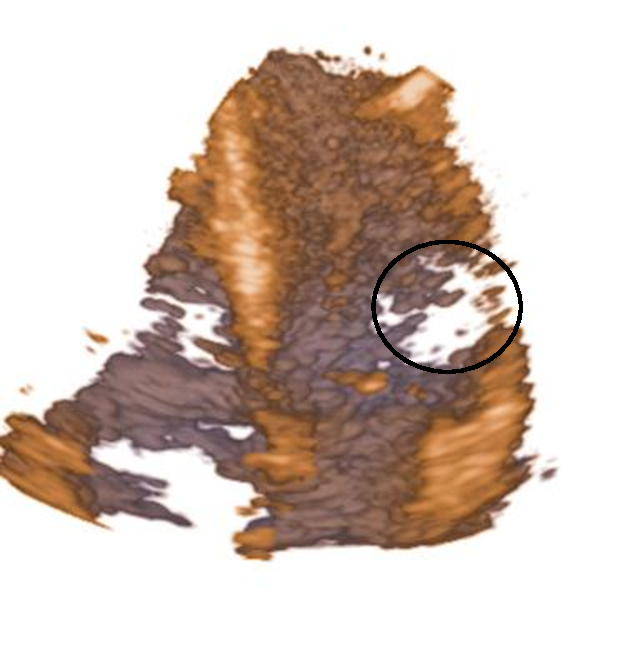
\includegraphics[height=0.4\textwidth]{global_otf_crown.pdf}\\
(a) & (b)\\
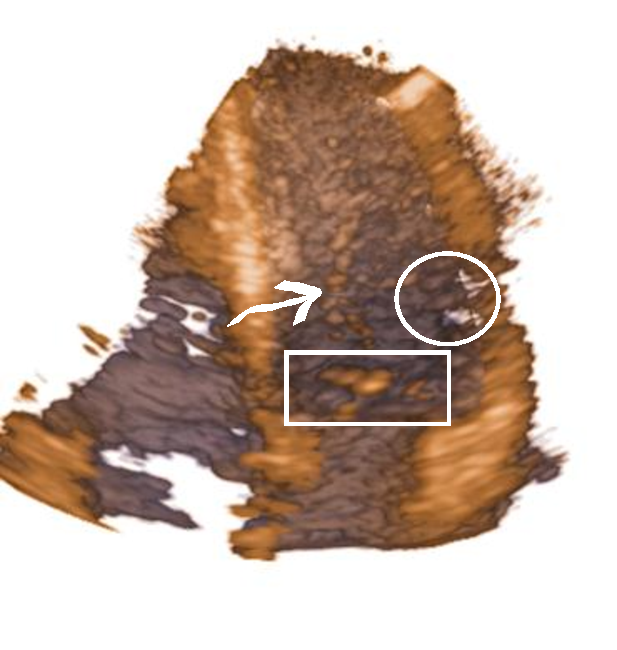
\includegraphics[height=0.4\textwidth]{regional_otf_c05_crown.pdf} & 
\includegraphics[height=0.4\textwidth]{residualGraphVsC.eps}\\
(c) & (d)
\end{tabular}
\end{center}
\caption[example] { \label{fig:vis} a) Global OTF with a low opacity threshold $\tau$. A lot of noise is visible inside the LV (circle). b) Global OTF with $\tau$ corresponding to the lowest MAE in Figure d. The image contains less noise, but also a large tissue dropout (circle). c) Blood pool based regional adaptive OTF with c=0.5 which is close to the minimum in d. The papillary muscle is now more visible (arrow) and the tissue dropout (circle) is smaller without pruning the mitral valve (sqare).  d) Parameter exploration in the view shown in a, b and c. MAE is plotted versus the $c$-value. For comparison, the global OTF has been converted into a function of $c$ using the global mean and standard deviation.}
\end{figure} 

Figures \ref{fig:vis}a, b and c show three renderings of the same apical 4-chamber view of one subject. With a low opacity threshold (Figure \ref{fig:vis}a), a lot of clutter noise is picked up in the apex of the LV (circle). With a threshold corresponding to the minimum MAE in Figure \ref{fig:vis}d, the clutter noise is removed (Figure \ref{fig:vis}b), but a tissue dropout (circle) has now increased in size. With the blood-pool based method (Figure \ref{fig:vis}c) clutter noise inside the LV is suppressed, giving a clear view of the endocardial tissue and a papillary muscle (arrow) without reducing the thickness of the mitral valve (square). The extent of the mentioned dropout is also reduced (circle). In Figure \ref{fig:vis}d we present a parameter exploration of the $c$-value introduced with the regional adaptive OTF. For comparison the global opacity threshold is substituted with a function of $c$, global mean and standard deviation. The figure shows that for a given view the MAE measure has a local minimum for both the global and regional methods, and that the regional OTF has a smaller MAE than the global OTF for all $c$.

% show spatial regularization

\section{Discussion}
% summarising contribution
A regional adaptive OTF based on blood-pool statistics has been proposed. The purpose was to better handle the high variation of signal within tissue as well as variability of noise signal inside the blood pool. Both quantitative and qualitative results reported in Section \ref{sec:res} shows that this has been accomplished. 

% Discuss quantitative results
We believe that the significant reduction in MAE for the regional adaptive method in Table \ref{tab:stat1} is caused by a reduced amount of rendering outliers. By outliers we mean rendering rays that stop far away from the endocardial boundary depicted by the reference segmentation, thus having a high absolute error. We observe that the difference in MAE in millimetre is small, between 1.5 and 2.5 mm for the three views in Table \ref{tab:stat1}, compared to normal average end-diastole myocardial thickness (around 10mm). However, regional improvements in order of centimetres can be observed in Figure \ref{fig:vis}c (circle). These large improvements are smoothed out by the MAE measure, but remains as a significant statistical improvement ($p<0.001$) in MAE-difference between the regional and global adaptive method in all three views (Table \ref{tab:stat1}).

% Discuss qualitative results
Table \ref{tab:stat2} shows that in 46 pair of renderings the regional adaptive OTF based on blood pool statistics provided renderings with less tissue dropouts and spurious structures inside the blood pool. However, Table \ref{tab:stat2} also shows that the regional adaptive method was ranked worse in the MV view for two subjects, and in four MV-views the two methods were equal. On the other hand, the MV statistics in Table \ref{tab:stat1} are the most significant among the three views. One explanation to these diverging results is: When doing the qualitative assessment the physician echocardiographer watched the whole cardiac cycle, where the statistics in Table \ref{tab:stat1} are calculated from a single end-diastolic frame. In end-diastole the mitral valve is closed, which means that the MV is outside our tracking model and therefore not included in the blood pool statistics. When the MV is inside the tracking model, thus included in the estimates, visual artefacts can occur since the MV will be treated as being a part of the blood pool and might get rendered transparent. %It is important to prevent this, given the high clinical value that the MV represent. 
Another explanation is that all the recordings are from an apical imaging view. From this view the MV is normal to the ultrasound beam. The MV has because of this better image quality than e.g. the LV endocardium and thus less variation is observed in the MV-view statistics than for the long-axis views (Table \ref{tab:stat1}). When the image quality is good it is hard to make any regional improvement compared with a global OTF. Opposite, the endocardial boundary has usually lower image quality than the MV from the apical imaging window. For the two 4-chamber views the statistics therefore has higher variation and for the inverted 4-chamber, that had large acoustic dropouts in many of the recordings, the improvement is much larger. 

% Discuss example renderings
The images in Figure \ref{fig:vis} demonstrate that our regional adaptation of the OTF provides a better tradoff between artificial tissue dropouts and spurious structures compared with a global OTF. In Figure \ref{fig:vis}d this improvement is quantified as $\textrm{MAE}_{global}(c) > \textrm{MAE}_{regional}(c), \forall c\in[-1.5, 1.5]$. This illustrate our findings that the global OTF did not produce a smaller MAE than the regional OTF in any pair of renderings if both methods where tuned to the lowest MAE. The gentle slope of $\textrm{MAE}_{regional}(c)$ in Figure \ref{fig:vis}d is another important observation. This indicates that the proposed method is less sensitive to changes in c, and therefore less tuning is often required. This observation was also done by the physician echocardiographer. 
The rendering in Figure \ref{fig:vis}c has a c-value corresponding to the minimum of $\textrm{MAE}_{regional}(c)$ in Figure \ref{fig:vis}d. We have often found the c-value at the local minimum of the MAE measure to be approximately the same c-value as both we and the physician echocradiographer would have selected in a given view. A fully automatic method could therefore iterate towards the local minimum by steepest descent, removing the need for manual tuning of $c$. It should be kept in mind that the success of this approach highly depends on a correct segmentation of the LV. This approach will also not be real-time, since an accurate segmentation of the LV usually involves manual adjustments and processing times in the order of seconds. One option is to use the real-time acquired LV delineation, used to estimate blood pool statistics, to measure rendering accuracy as well. A different endocardial detection scheme should then be used to estimate blood-pool statistics, to avoid a too close coupling between the LV delineation used for estimation and validation. 

%Discuss spatial and temporal smoothing
As mentioned, no spatial regularization was applied to the results in Section \ref{sec:res}. However, spatial smoothing will decrease the variation in $\tau_r$ across the image, and with increased filter kernels the results will become equivalent to applying an OTF with a global adaptive opacity threshold $\tau_g$ based on the whole blood pool. With increased spatial smoothing less visual artefacts have been observed at the cost of a higher MAE. As no flickering has been observed, temporal smoothing had no positive effect. E.g. the rapid movement of the mitral valve caused artificial dropouts in all views when temporal smoothing was applied. 

\subsection{Limitations}
The choice of using a deformable model to indicate the blood pool location imposes some limitations for the proposed method. As mentioned, some important cardiac structures are included in the depicted blood pool and might result in visual artefacts. However, how the LV endocardial boundary is derived is not relevant for the result in this paper. Local edge detectors combined with regularization may work equally well for limiting the regional estimation of means and standard deviations to the blood pool.


%Caused by the decision of using a deformable model to indicate the blood-pool location.

\section{Conclusion}
%Many adaptive algorithms for DVR have been proposed in the literature, however they are usually tested on data with considerably higher SNR than ultrasound. We have proposed a method for fast adaptive visualization of low-SNR cardiac 3D ultrasound. Compared with a global OTF we have shown that the regional adaptive method, based on blood pool statistics, is capable of providing a better tradeoff between tissue dropouts and the number of spurious structures inside the blood pool. The need for manual tuning is reduced by adapting the OTF to the data at hand, potentially leading to a fully automatic, data-dependent OTF.
In this paper we have introduced and investigated an adaptive DVR method for real-time visualization of cardiac 3D ultrasound. Compared to a global OTF we have shown, both with quantitative and qualitative results, that the regional adaptive method, based on blood pool statistics, is capable of reducing tissue dropouts and spurious structures inside the blood pool. The need for manual tuning is reduced by adapting the OTF to the data at hand, potentially leading to a fully automatic and data-dependent OTF.
